\documentclass[a4paper,12pt]{article}
\usepackage[a4paper, total={180mm, 272mm}]{geometry}

\usepackage{fontspec}
\setmainfont[Path=fonts/, Extension=.ttf]{ipaexm}

\setlength\parindent{3.5em}
\setlength\parskip{0em}
\renewcommand{\baselinestretch}{1.247}

\usepackage{epic}
\usepackage{eepic}
\usepackage{xcolor}

\usepackage{graphicx}
\graphicspath{{images/}}

\begin{document}

\thispagestyle{empty}

\Large
\noindent \\
Motion Wind Ino\medskip
\par
\normalsize
Add the effect of wind flow lines to the picture\\
\par
For animation, it uses a fine arts drawing method to represent the reference to wind.\par
In the wake of the bright peak portion from the RGB value of the pixel,\par
you can add effects, such as flowing in color.\\
\\
-{-}- \ Inputs \ -{-}-\\
Source\par
Connect the image to process.\\
Reference\par
Connect the reference image to put the strength of the effect into each Pixel.\\
\\
-{-}- \ Settings \ -{-}-\\
Direction\par
Specify the direction of the flow line.\par
The only directions are above (Up) under (Down) left (Left) right (Right).\par
The default setting is right (Right).\par
Direction, is a fixed direction as viewed from the camera. For the slope of the image\par
it is not possible to tilt the direction by rotation or camera Z rotation etc.\par
of the image using (Geometry conversion),\par
please take note.\\
\\
Dark\par
When OFF it will be streamlined the bright parts of the image.\par
When ON it will be streamlined to the dark parts of the image.\par
The default setting is OFF.\\
\\
Alpha Rendering\par
This is a valid switch only when there is an Alpha channel.\par
When OFF, it masks the changes in the RGB values using the Alpha value.\par
When ON, the process is also applied to the Alpha.\par
The default setting is ON.\\
\\
Length Min\\
Length Max\par
Specify the length of the flow line.\par
The unit is millimeters.\par
Specify a value greater than or equal to 0. The maximum is 1000.\par
The following specified points, will have subtle changes in the length.\par
If you give a different values, the length between the values will change randomly.

\newpage

\thispagestyle{empty}

\ \vspace{-0.2em}
\par
With the same values, it will no longer use randomness and will be the same length.\par
The default values for Min (minimum value) is 0, and Max (maximum value) is 18.\par
-{-}> \textquotedbl Motion Wind Figure 1 \ \ Length Wind\textquotedbl \ reference\par
-{-}> \textquotedbl Motion Wind Figure 4 \ \ Force is 1 and Density is 1\textquotedbl \ reference\par
-{-}> \textquotedbl Motion Wind Figure 7 \ \ Length Wind and Force is 10\textquotedbl \ reference\\
\\
Length Bias\par
This changes the offset of the random pattern for the length.\par
Using a value between 0.1 and 1.0, will make it more short,\par
If you specify a value of 1.0 it will make the randomness become uniform,\par
Using a value between 1.0 and 10.0, increases the length to be longer.\par
Specify how you would like it to look.\par
The default value is 1.\par
-{-}> \textquotedbl Motion Wind Figure 1 \ \ Length Wind\textquotedbl \ reference\\
\\
Length Seed\par
This changes the random pattern for the length.\par
Specify an integer value greater than or equal to 0.\par
If you give the same value to the same image, it will reproduce the same pattern.\par
Change the value if you want a different pattern.\par
For example, in the Fix of the movie, when you want the pattern to change\par
streamlines, on a frame-by-frame basis, change the seed value.\par
The default value is set to 1.\\
\\
Force Min\\
Force Max\par
Specify the start momentum of the flow.\par
A value between 0.1 and 1.0, will immediately decay for a weak momentum,\par
If you specify a value of 1.0 it will be attenuated to linear momentum,\par
Between 1.0 and 10.0, will make a not quite attenuated strong momentum,\par
specify how you would like it to look.\par
If you give different values, momentum between the values will change randomly.\par
With the same values, it will no longer be random and will use the same momentum.\par
The default value is 1 for both.\par
-{-}> \textquotedbl Motion Wind Figure 2 \ \ Force Wind\textquotedbl \ reference\par
-{-}> \textquotedbl Motion Wind Figure 5 \ \ Force is 0.1\textquotedbl \ reference\par
-{-}> \textquotedbl Motion Wind Figure 7 \ \ Length Wind and Force is 10\textquotedbl \ reference\\
\\
Force Bias\par
This changes the offset of the random pattern for the momentum.\par
Using a value between 0.1 and 1.0, will make it become more weak,\par
if you specify a value of 1.0 it will make the randomness become uniform,

\newpage

\thispagestyle{empty}

\ \vspace{-0.2em}
\par
using a value between 1.0 and 10.0, will make it become more strong.\par
Specify how you would like it to look.\par
The default value is 1.\par
-{-}> \textquotedbl Motion Wind Figure 2 Force Wind\textquotedbl \ reference\\
\\
Force Seed\par
This changes the random pattern for the momentum.\par
The options are similar to \textquotedbl Length Seed\textquotedbl .\\
\\
Density Min\\
Density Max\par
Specify the concentration of the streamline.\par
There is no streamlined effect when the value is 0,\par
Using values between 1.0 and 0.0, will make it become thinner,\par
The reference concentration is a value of 1.0,\par
using a value greater than 1.0, will make it become darker. The maximum is 100.\par
If you give different values, concentration between the values will change randomly.\par
With the same values, it is no longer random and will use the same concentration.\par
The default value is 1 for both.\par
-{-}> \textquotedbl Motion Wind Figure 3 \ \ Density Wind\textquotedbl \ reference\par
-{-}> \textquotedbl Motion Wind Figure 6 \ \ Density is 0.2\textquotedbl \ reference\\
\\
Density Bias\par
This changes the offset of the random pattern for the concentration.\par
Using a value between 0.1 and 1.0, the concentration is increased,\par
if you specify a value of 1.0 it will make the randomness become uniform,\par
using a value of between 1.0 and 10.0, will make it become more dark.\par
The default value is 1.\par
-{-}> \textquotedbl Motion Wind Figure 3 \ \ Density Wind\textquotedbl \ reference\\
\\
Density Seed\par
This changes the random pattern of the concentration.\par
The options are similar to \textquotedbl Length Seed\textquotedbl .\\
\\
Rather than streamline, to use a uniform flow effect\par
\ \ \textquotedbl Length Min\textquotedbl \ and \textquotedbl Length Max\textquotedbl 、\par
\ \,\, \textquotedbl Force Min\textquotedbl \ and \ \, \textquotedbl Force Max\textquotedbl 、\par
\textquotedbl Density Min\textquotedbl \ and \textquotedbl Density Max\textquotedbl 、\par
and give the same values to each for the picture rather than streamline for the flow.\\
\\
To synchronize a random pattern\par
一 Using sheets,

\newpage

\thispagestyle{empty}

\ \vspace{-0.2em}
\par
\noindent \hskip 7.4em length\_random\_seed、\par
\noindent \hskip 8em force\_random\_seed、\par
\noindent \hskip 7em density\_random\_seed、\par
Using the same values, patterns will grow the same, with the same timing,\par
and weakening amounts.\par
It will break apart from the pattern when using different values.\\
\\
To secure a random pattern when the camera is moving\par
When on the background image, using camera movement, a random pattern\par
for each frame in accordance with the change of the picture will occur.\par
If you want to fix the pattern it must be multiplied by the processing\par
in the entire background image.\\
-{-}-{-}-{-}\\
Length Ref\par
When OFF it will not be referred to.\par
When ON, this refers to the image, and will give it a length.\par
Specifying the reference, will give the length to the Red channel of the image.\par
When not specified, it will give the length to the brightness of the image.\par
The darker the Pixel when the streamline begins, will make it become shorter.\par
The whole image tone is weakened, please adjust the length values\par
specified in (Min, Max).\par
The default setting is OFF.\\
\\
Force Ref\par
When OFF it will not be referred to.\par
When ON, the refers to the image, and will give it strength.\par
Specifying the reference, will give the strength to the Red channel of the image.\par
When not specified, it will give the strength to the brightness of the image.\par
The darker the Pixel when the streamline begins, will make it become weaker.\par
The whole image tone is weakened, please adjust the momentum values\par
specified in (Min, Max).\par
The default setting is OFF.\\
\\
Density Ref\par
When OFF it will not be referred to.\par
When ON, the refers to the image, and will give it light and dark shade.\par
Specifying the reference, will give the shade to the Red channel of the image.\par
When not specified, it will give the shade to the brightness of the image.\par
The darker the Pixel when the streamline begins, will make it become thinner.\par
The whole image tone is weakened, please adjust the concentration values\par
specified in (Min, Max).\par
The default setting is OFF.

\newpage

\thispagestyle{empty}

\ \vspace{1.3em}
\par
\noindent Reference\par
Choose how Reference image values put the strength of the effect into each Pixel.\par
An image is connected to the \textquotedbl Reference\textquotedbl \ of the input,\par
Choose from Red/Green/Blue/Alpha/Luminance/Nothing.\par
Choose Nothing when you do not want this effect, it will turn off the connection.\par
The default setting is Red.

\newpage

\thispagestyle{empty}

\ \vspace{-0.2em}
\par
\noindent Motion Wind Figure 1 \ \ Length Wind

\large
\noindent \begin{picture}(0,0)
\linethickness{0.01em}
\put(1,-198.5){\line(1,0){198}}
\put(9,-200.5){\line(0,1){62}}
\drawline[0](9,-143)(193,-198.5)
\drawline[0](9,-143)(102,-198.5)
\drawline[0](9,-143)(28,-198.5)
\put(0.5,-135){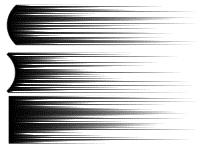
\includegraphics[width=13.9em]{MotionWindInoFunction1LengthWindA}}
\put(142,-171.5){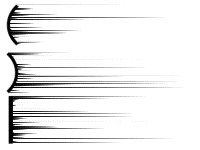
\includegraphics[width=13.9em]{MotionWindInoFunction1LengthWindB}}
\put(284.5,-200){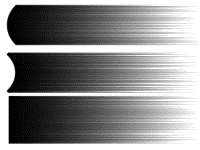
\includegraphics[width=13.9em]{MotionWindInoFunction1LengthWindC}}
\put(209,-16.5){\normalsize{Bias is 0.1}}
\put(351,-45){\normalsize{Bias is 10}}
\end{picture}\\[12.6em]

\normalsize
\noindent Motion Wind Figure 2 \ \ Force Wind

\large
\noindent \begin{picture}(0,0)
\linethickness{0.01em}
\put(1,-198.5){\line(1,0){198}}
\put(9,-200.5){\line(0,1){62}}
\drawline[0](9,-143)(193,-198.5)
\spline(9,-143)(129,-150)(188,-180)(195,-198.5)
\spline(9,-143)(20,-168.5)(85,-192.5)(193,-198.5)

\put(0.5,-135){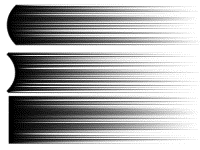
\includegraphics[width=13.9em]{MotionWindInoFunction2MotionWindA}}
\put(142,-171.5){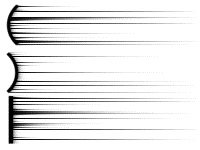
\includegraphics[width=13.9em]{MotionWindInoFunction2MotionWindB}}
\put(284.5,-200){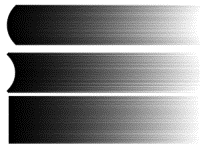
\includegraphics[width=13.9em]{MotionWindInoFunction2MotionWindC}}
\put(209,-16.5){\normalsize{Bias is 0.1}}
\put(351,-45){\normalsize{Bias is 10}}
\end{picture}\\[12.65em]

\normalsize
\noindent Motion Wind Figure 3 \ \ Density Wind

\large
\noindent \begin{picture}(0,0)
\linethickness{0.01em}
\put(1,-198.5){\line(1,0){198}}
\put(9,-200.5){\line(0,1){62}}
\drawline[0](9,-143)(193,-198.5)
\drawline[0](9,-166.5)(193,-198.5)
\drawline[0](9,-192)(193,-198.5)

\put(0.5,-135){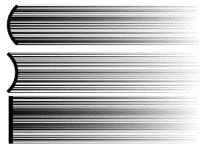
\includegraphics[width=13.9em]{MotionWindInoFunction3DensityWindA}}
\put(142,-171.5){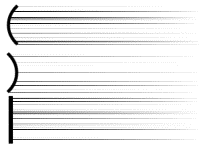
\includegraphics[width=13.9em]{MotionWindInoFunction3DensityWindB}}
\put(284.5,-200){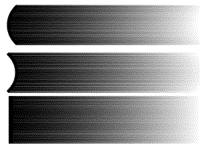
\includegraphics[width=13.9em]{MotionWindInoFunction3DensityWindC}}
\put(209,-16.5){\normalsize{Bias is 0.1}}
\put(351,-45){\normalsize{Bias is 10}}
\end{picture}

\newpage

\thispagestyle{empty}

\ \vspace{-0.1em}
\par
\large
\noindent \hskip 10.5em Length Min equal Max Wind\\[-0.15em]
\normalsize
Motion Wind Figure 4 \ \ Force is 1 and Density is 1

\large
\noindent \begin{picture}(0,0)
\put(28.5,-132){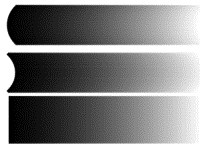
\includegraphics[width=13.9em]{MotionWindInoFunction4}}
\end{picture}\\[7.6em]

\large
\noindent \hskip 10.5em Length Min equal Max Wind\\[-0.15em]
\normalsize
Motion Wind Figure 5 \ \ Force is 0.1

\large
\noindent \begin{picture}(0,0)
\put(28.5,-132){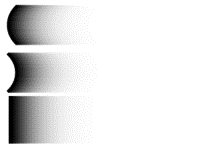
\includegraphics[width=13.9em]{MotionWindInoFunction5}}
\end{picture}\\[7.6em]

\large
\noindent \hskip 10.5em Length Min equal Max Wind\\[-0.15em]
\normalsize
Motion Wind Figure 6 \ \ Density is 0.2

\large
\noindent \begin{picture}(0,0)
\put(28.5,-132){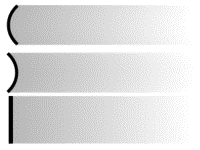
\includegraphics[width=13.9em]{MotionWindInoFunction6}}
\end{picture}\\[7.4em]

\normalsize
\noindent Motion Wind Figure 7 \ \ Length Wind and Force is 10

\large
\noindent \begin{picture}(0,0)
\put(28.5,-132){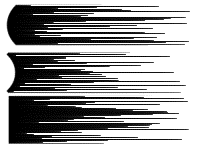
\includegraphics[width=13.9em]{MotionWindInoFunction7}}
\end{picture}

\end{document}